% !TeX TS-program = xelatex
% !Mode TeXUTF-8
%# -- codingutf-8 --
% !TeX encoding = UTF-8
%%%%%%%%%%%%%%%%%%%%%%%%%%%%%%%%%%%%%%%
\zihao{-4}
%---------------------------------------
\chapter{关于模板的一些说明}%\label{chpt:1}
%---------------------------------------
本模版\glossary{模板}是为{\university\school}本科毕业生撰写毕业论文而设计的，版面尺寸按照{\university}的论文撰写要求选取~\cite{moban_fujian}。模板的第一版是
2006年完成的，经过多年的使用、 改进，最终发展成目前的版本。

模板的最近一次修改是2024年8月。 这次修改的变动比较大，首先 \university 对论文的结构、格式和要求进行了比较大的改动~\cite{moban_wenjian,moban_fujian}；其次，为了适应更多的使用者，本次模板的编译采用的是 XeLatex，不是以前的 PdfLatex。

第一次使用本模版时，请先阅读~\ref{subsec:1}节；%如果安装\CTeX{}\index{\CTeX} 有问题，请阅读~\ref{sec:versionSelect}节；
如果对数学公式、符号或定义、定理、证明等各种命令环境不熟悉，请阅读第~\ref{sec:2two}
节；如果对表格或图形的\index{图形插入}插入不熟悉，请阅读第~\ref{sec:ssss} 节；如果对\index{交叉引用}交叉引用不熟悉，请阅读第~\ref{sec_si4}节。 如果想了解在~\LaTeX 中\index{程序引入}引入程序代码，如
~{\tt Matlab}\index{Matlab}，{\tt Mathematica}\index{Mathematica}, {\tt Python}\index{Python}，{\tt R}\index{R} 和~{\tt C/C++}\index{C/C++} 等的代码，请阅读第~\ref{sec:codeinludsion}节, 并分别参考附录~\ref{appendix:A}、\ref{appendix:B}、\ref{appendix:E}、\ref{appendix:C}、\ref{appendix:D} 中的实例. 
\section{模板的构成}\label{subsec:1}
本模板由若干文件组成，所有文件都存放在一个主文件夹\index{文件夹}里。为了使用和管理方便，在主文件夹中又分了七个子文件夹：{\tt preample, codes, tables，declaration，zhengwen, fujian, wenxian}，其中~{\tt preample\index{文件夹!preample}, tables\index{文件夹!table}, declaration\index{文件夹!declaration}} 中的文件一般不用管。子文件夹~{\tt codes} 中放有一些制作本说明时的附件所用的一些代码文件，如果不需要可以删除。
%而~{\tt codes\index{文件夹!codes}} 在熟悉模板后可以删除。文件夹~{\tt fujian\index{文件夹!fujian}} 包含中英文摘要及附录，文件夹~{\tt declaration\index{文件夹!declaration}} 中是独创性声明，而文件夹~{\tt wenxian\index{文件夹!wenxian}} 则包含一个参考文献列表文件。模板由主文件~{\tt mytemplate.tex\index{mytemplate.tex}} 及五类子文件构成：
\begin{description}
  \item[主文件~mytemplate:] 论文的编译一般通过主文件进行。学生的基本信息，如姓名，学号，论文题目等，都在主文件上输入。主文件名可根据自己的需求改动。
  \item[文件夹~codes:]\label{item:codes} 文件夹中包含几个程序代码。如果使用者自己没有代码，可以将其删除。
  \item[文件夹~zhengwen:] 文件夹中包含五个文件，分别对应五章。使用者可以根据自己论文的实际章数来增加或减少这里的文件数，同时录入自己论文相应章节的内容。
  \item[文件夹~fujian:] 文件夹中包含以下几个文件：
  \begin{enumerate}
  	\item {\tt abstract.tex\index{abstract.tex}}，这是论文的摘要。
  	\item {\tt thanks.tex\index{thanks.tex}}，这是论文的致谢词部分。
  	\item {\tt fulu\index{文件夹!fulu.tex}}, 这是论文附录的引入文件。使用者如果没有附录，那就将附录文件~{\tt fulu}删除。
  \end{enumerate}
  \item[文件夹~wenxian:]文件夹中包含一个文件，其中是论文中所引用的参考文献。
\end{description}
%  \item\label{item:2} 这一类文件是论文的主要组成部分，由学生完成。有以下几个文件：
%  \begin{enumerate}
%    \item {\tt abstract.tex\index{abstract.tex}}，这是论文的摘要。
%    \item {\tt body.tex\index{body.tex}}，这是论文的正文部分。
%    \item {\tt bibfile.tex\index{bibfile.tex}}，这是论文的参考文献。
%    \item {\tt thanks.tex\index{thanks.tex}}，这是论文的致谢词部分。
%  \end{enumerate}
%  以上两类文件都存放在主文件夹里，学生只须在相关的文件中按~\LaTeX\index{\LaTeX} 的要求及文件中的提示输入相应的内容即可。
%  \item 这一类是三个与教师有关的文件：
%  \begin{enumerate}
%    \item\label{term1} {\tt zhidaojiaoshigeifen.sty}，这个文件包含指导教师评分及评阅意见，由指导教师完成。
%    \item {\tt jiaochageifen.sty}，这个文件包含交叉评阅意见及评分，由负责交叉评阅的教师完成。
%    \item {\tt dabianchengji.sty}，这个文件包含答辩评审意见、答辩分数及论文成绩，由教师答辩小组组长完成。
%  \end{enumerate}
%  这类文件存放在子文件夹~{\tt filesforteachers} 中。相关教师只须在对应的文件中按\LaTeX
%  的要求及文件中的提示输入相应的内容即可。具体的对应文件及填写方法参看后面表格(开题报告二，教师评阅表，交叉评阅表，答辩记录表)中的说明。
%  \item 这一类有两个个文件：
%  \begin{enumerate}
%    \item {\tt kaitibaogao.tex}（开题报告）；
%    \item {\tt dabianjilu.tex\index{dabianjilu.tex}}（答辩记录）。
%  \end{enumerate}
%   这类文件存放在子文件夹~{\tt filesforstudent} 中。第一个文件用来填写开题报告的具体内容，后一个文件是用来填写答辩的记录内容。完成人只须在对应的文件中按~\LaTeX 的要求及文件中的提示输入相应的内容即可。
%   具体的对应文件及填写方法参看后面表格（开题报告一，第开题报告二，答辩记录表）中的说明。
%  \item\label{item:4} 这一类是三个与教师有关的文件：
%  \begin{description}
%    \item\label{term1} {\tt zhidaojiaoshigeifen.tex\index{zhidaojiaoshigeifen.tex}}，这个文件包含指导教师评分及评阅意见，由指导教师完成。
%    \item {\tt jiaochageifen.tex\index{jiaochageifen.tex}}，这个文件包含交叉评阅意见及评分，由负责交叉评阅的教师完成。
%    \item {\tt dabianchengji.tex\index{dabianchengji.tex}}，这个文件包含答辩评审意见及论文评定成绩，由教师答辩小组组长完成。
%  \end{description}
%  这类文件存放在子文件夹~{\tt filesforteachers} 中。具体操作时，学生可以将相关的文件发给相关教师，相关教师只须在对应的文件中按~\LaTeX
%  的要求及文件中的提示输入相应的内容，然后发还给学生，学生用其替换原来的同名文件再通过主文件编译即可。具体的对应文件及填写方法参看后面表格（开题报告二，指导教师评阅表，交叉评阅表，答辩记录表）中的说明。
%  \item\label{item:head} 这一类中除头文件{ \tt SWUthesis.sty\index{SWUthesis.sty}} 外还有一些诸如学校的~logo 和学院的~logo 之类的文件。
%        这几个文件单独放在子文件夹~{\tt preample} 中，这些文件一般不用改动。
%
%      这四类文件在前面相关的内容录入后，通过编译主文件，会自动将指导教师评阅意见，交叉评阅意见以及答辩记录，答辩分数和论文等级等相关的内容导入对应表格，最后生成~PDF 格式的文件。
%  \item\label{item:miscellanceous} 这一类中有六个文件：{\tt coverpage.tex\index{coverpage.tex}}（封面），
%  {\tt kaiti\_1.tex\index{kaiti\_1.tex}}（开题报告表格的前半部分），{\tt kaiti\_2.tex\index{kaiti\_2.tex}} （开题报告表格的后半部分），
%  {\tt pingyue\_1.tex\index{pingyue\_1.tex}}（指导教师评阅表）， {\tt pingyue\_2.tex\index{pingyue\_2.tex}} （交叉评阅表），
%        {\tt dabian.tex}（答辩记录表）。这几个文件，单独放在子文件夹~{\tt tables} 中，它们只生成封面或表格的框架，其中需要填入的内容通过编译会自动从其它相关文件中导入，
%        所以一般不用对这些文件做改动。
%\end{enumerate}
%总之第~\ref{item:head} 类和第~\ref{item:miscellanceous} 类的文件一般不用去管，主文件和~\ref{item:2}--~\ref{item:4} 类中的子文件在完成后由学生统一通过主文件编译，
%最后生成包含所有内容和所有表格的、完整的论文的~PDF 格式的文件。子文件夹~{\tt codes} 中放有一些制作本说明时所用的一些文件，如果不需要可以删除。
\subsection{三级标题}
\fbox{本节为测试三级标题在目录中的显示而设。}
\section{\TeX 简介\index{\TeX}}
\TeX 是计算机科学家、图灵奖\index{图灵奖}得主~Knuth\index{Knuth} 教授设计的一款权威的科技论文排版软件！学习~\TeX(\LaTeX)，
Knuth 的专著~\cite{knuth} 无疑是权威之选。该书排版堪称完美，从中可以看出大师的魅力。更重要的是~Knuth 教授无偿公开了~\TeX{} 的所有源代码，
也就是说它是开源 (Open Source)的（通俗地说就是可以免费使用）。正因为这个原因，后人在其基础上开发了~\LaTeX 。\LaTeX 方便好用，被广泛传播，成了当今世界科技界最权威的论文排版软件。
作为一个非常全面的~\LaTeX{} 的参考书，\cite{companion} 是一个不错的选择。如果阅读英文有困难，作为一个初学者，也可以先看看~\cite{zhanglibo}。

\TeX{} 和~\LaTeX{} 排版软件和~MS 的~Word \index{Word}软件不同，后者是``所见即所得\index{所见即所得}"(WYSIWYG\index{WYSIWYG}，what you see is what you get)，而前者是``所想即所得\index{所想即所得}"(WYWIWYG\index{WYWIWYG}，what you want is what you get)。
二者在风格上迥然不同，因此学习~\LaTeX{} 需要稍微改变一下自己的习惯。

%\paragraph{Run-in headings.}
国内较早使用的~\LaTeX 汉化版\index{\LaTeX 汉化版}是~
\CTeX，可在~\href{http://www.ctex.org}{\CTeX{} 网站}~\index{\CTeX 网站}免费下载安装。\CTeX{} 安装包自带了一个编辑器~WinEdt\index{WinEdt}, 不过这个编辑器需要注册；否则会频繁跳出弹窗，提示你注册，很是烦人！可以用~\href{https://texstudio.sourceforge.net/}{TeXstudio} \index{TeXstudio} 作为编辑器来替代~WinEdt。这时需要将~TeXstudio 和\CTeX 的编译器关联起来，当然也可以选择 TexLive + TeXstudio 的组合。TexLive\index{TexLive} 可以从清华大学的~\href{https://mirrors.tuna.tsinghua.edu.cn/CTAN/systems/texlive/Images/}{镜像网站}下载。

%---------------------------------------
\section{\LaTeX{} 文件的编译\index{\LaTeX 文件的编译}}
%---------------------------------------
\LaTeX{}的编译器\index{编译器}有多个，为了避免不必要的麻烦，本模板的编译指定采用~{\tt XeLatex}\index{XeLatex}. 因此用其它编译器编译就会报错. 另外，源文件如果是用其它编辑器录入的, 在用~TeXsdudio 打开保存之前请确认其是采用的是~UTF-8 \index{UTF-8}汉字编码\index{汉字编码}，否则文件可能会出现乱码. 可以先用记事本\index{记事本}将文件打开, 点击``文件", 在下拉菜单中选择``另存为"后会弹出一个如图~\ref{fig:ansi2utf8} 的窗口，在其下部``编码"的下拉窗口中选择``UTF-8", 然后点击保存既可转成UTF-8的编码.
\begin{figure}[ht]
  \centering
  % Requires \usepackage{graphicx}
  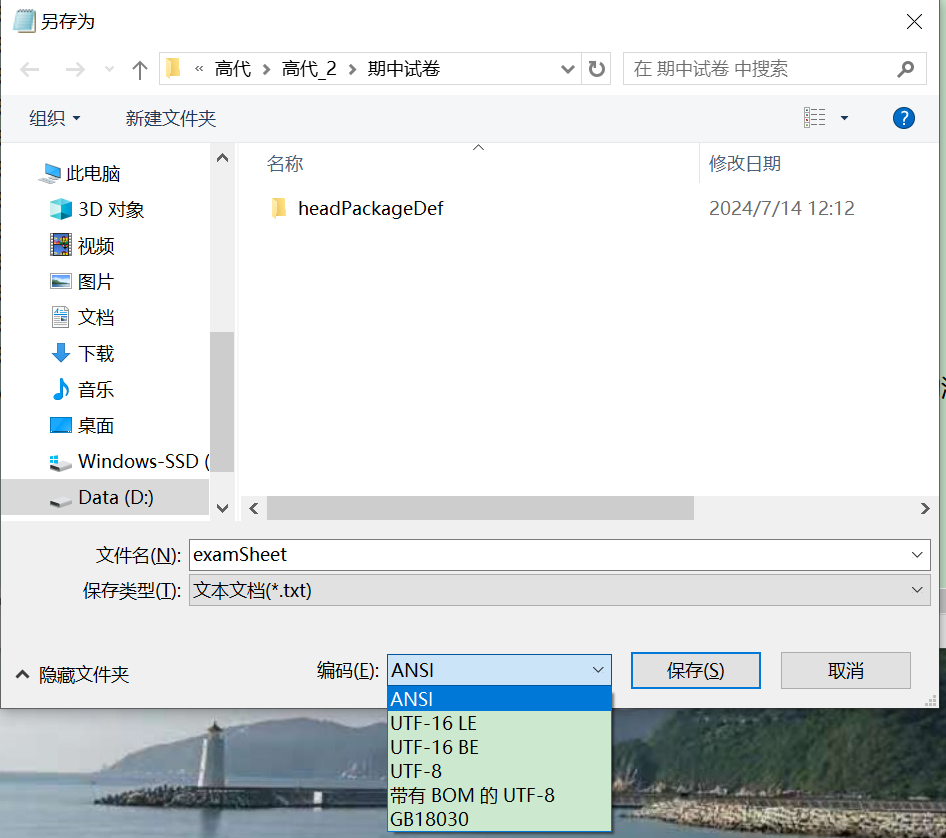
\includegraphics[width=12cm]{figs/ansi2utf8.png}\\
  \caption{ANSI编码转UTF-8编码}\label{fig:ansi2utf8}
\end{figure}
